\section{Design Pattern}
\label{sec:design-pattern}

The design pattern used is simply using the most intuitive as possible.
The most needed are creating interaction with \ac{BREAD} model, simple interface and interaction with mockup, and \ac{SPA}.
With these simple and general patterns, the development process can quickly go from visualized plan into actual implementation rather than going through a long conversion of requirements into design before.
What can be used here are for multiple purposes such as functionality, logic flow, visual or aesthetics.

% --------------------------------------------------
\subsection{{BREAD} Model}
\label{sec:bread-model}

\ac{BREAD} model consists of browse, read, edit, add, and delete, also including search by browse.
It is the most common basic functions of persistent storage in a software.
This is the minimum pattern that usual or general daily software can do based on user usage.
Although there are a lot of similar name with it, such as \ac{CRUD} and even \ac{SCRUD}, \ac{BREAD} can be more preferred if the software essentially not create a new thing, rather, add an existing thing but outside the software.
Related to knowledge management, it is more familiar and fit to ``add a knowledge'' than ``create a knowledge''.
As illustrated in \autoref{fig:bread-model}, it allows for:

\begin{easylist}
& Browse or search existing entries.
& Read the retrieved entries.
& Edit available entries.
& Add a new entry.
& Delete selected entries.
\end{easylist}

\begin{figure}[h]
    \centering
    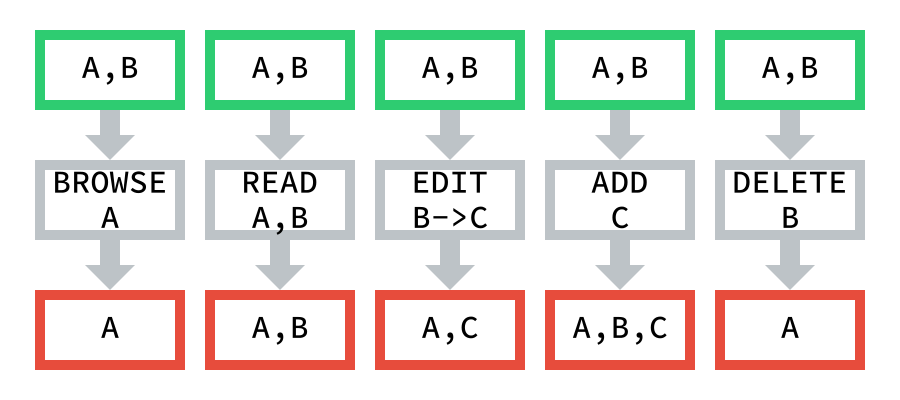
\includegraphics[width=8cm]{\dir/include/bread-model.png}
    \caption{Browse, Read, Edit, Add, Delete interaction}
    \label{fig:bread-model}
\end{figure}

For example purpose, let's say all data $A,B$ will go through \ac{BREAD} model operation.
If browse for $A$ from all data, then get just $A$.
If read $A,B$ from all data, then get $A,B$.
If edit $B$ in all data to $C$, then all data become $A,C$.
If add $C$ to all data, then all data become $A,B,C$.
If delete $B$ from all data, then all data become $A$.

% --------------------------------------------------
\subsection{Simple Interface and Interaction}
\label{ssec:simple-interface-interaction}

Particularly a very simple web app that doesn't require in depth logic explanation, can directly be planned in visual way of wireframe and mockup.
So that is what a simple interaction and interface can do and seen.
Wireframe is a typical way to put the bare essential elements (such as texts and images) onto a design, it contains all the information architecture.
It is a low fidelity design that shows the main software functionality without the aesthetics.
Mockup is a realistric representation to visualize the design, if the information architecture that needed has already present.
It is a middle to high fidelity design of how the software look, it basically more focus towards the aesthetics.
\autoref{fig:wireframe-mockup} is an example of an already built wireframe and mockup for some part of an application.
Mockup is closer to the actual or expected result especially the visual details of layout, color, and typography.

\begin{figure}[htbp]
  \centering
  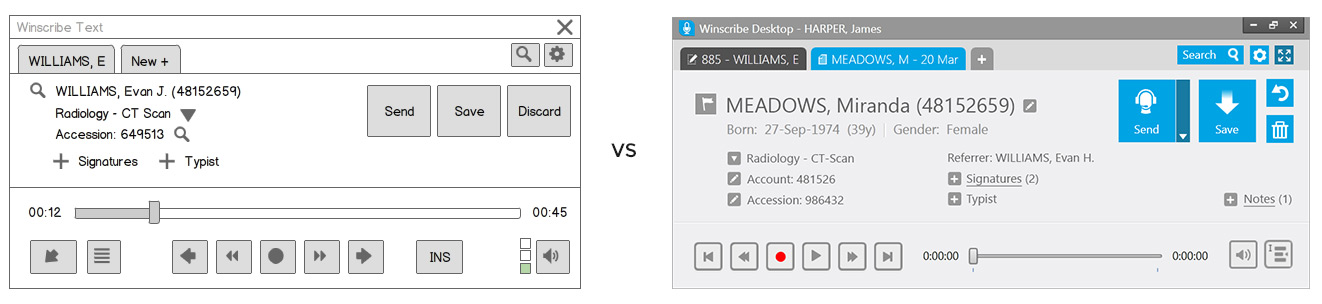
\includegraphics[width=\textwidth]{\dir/include/wireframe-mockup.jpg}
  \caption[Wireframe vs Mockup Example]{Example of wireframe vs mockup \autocite{Trentini2015WM}}
  \label{fig:wireframe-mockup}
\end{figure}

% --------------------------------------------------
\subsection{Single Page Application (SPA)}
\label{ssec:spa}

In actual user's view, a simple interaction and interface can use \ac{SPA}\index{SPA}\index{single page application} approach as the client app view.
\ac{SPA} model or design is a web application that can fits on a one web page, so all the codes can be retrieved with only a single page load, it is a contrary to the multi page application that has many pages or windows.
In \ac{SPA}, template of the page that already is utilized to contain then present only the required data rather than sending and receiving the whole page, so that its logic can also be represented simply like in \autoref{fig:spa}, which also compared with other model/design which is a common or traditional web app design.
It employs design from both application technology architecture and visual point of view.
Simply put, \ac{SPA} is not using multiple windows or pages to layout the interface, without the need to move around between some different places.

\begin{figure}[htbp]
  \centering
  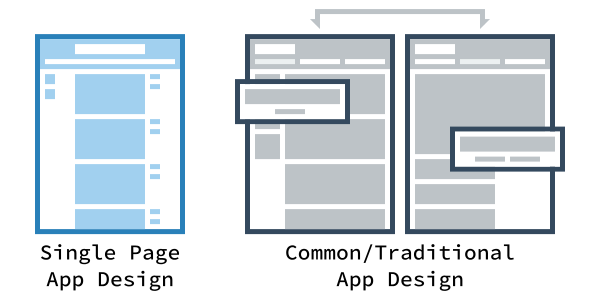
\includegraphics[width=10cm]{\dir/include/spa-design.png}
  \caption[Single Page Application design comparison]{Comparison of a Single Page Application design and other}
  \label{fig:spa}
\end{figure}
